\documentclass{article}
\setlength\parindent{0pt}
\usepackage[hmargin=1in,vmargin=1in]{geometry}
\setlength{\parskip}{.5em}
\usepackage{graphicx}

\title{CMPT 409 Assignment 6}
\author{Heather Li, Ekjot Singh Billing, Manshant Singh Kohli}

\begin{document}
\maketitle

\section{Bejeweled}
Completely Done
Bruteforce, at most (7*8)*2=112 swaps



\section{Binary}
Completely Done
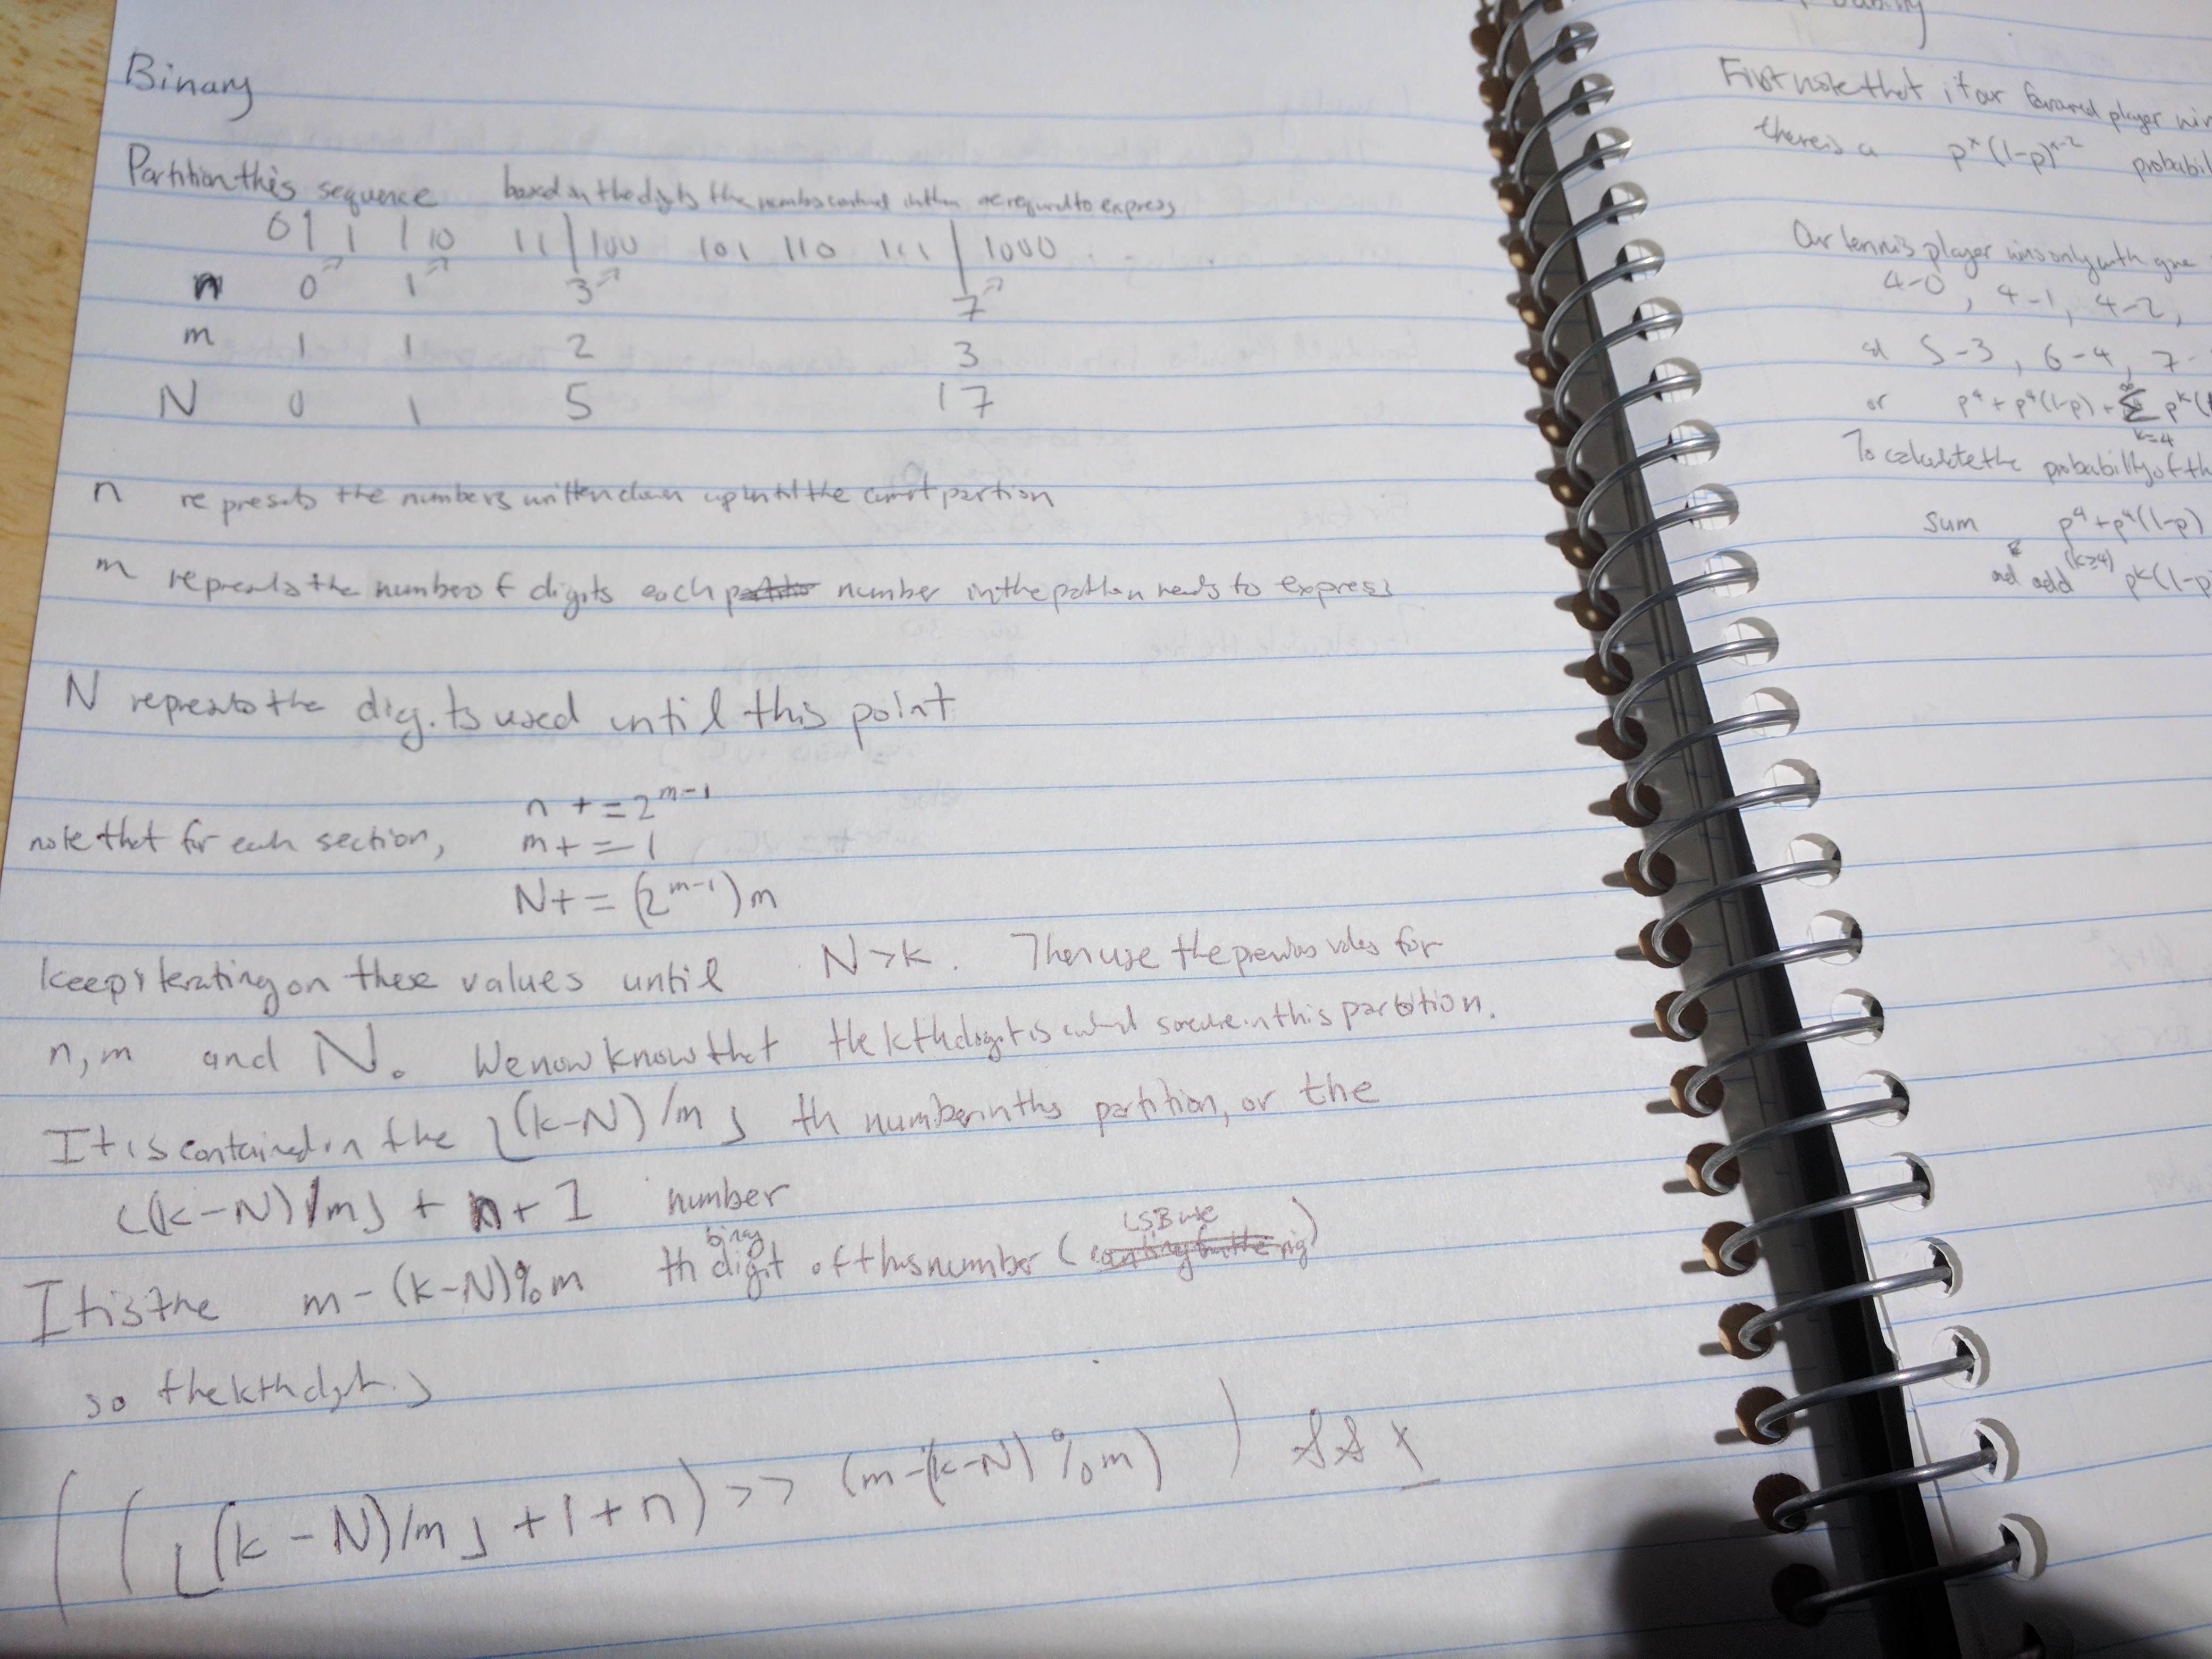
\includegraphics[width=.75\textwidth]{binary}

\section{City Slickers}
Kinda not really solution

There's probably something better than using shortest-path between ranches. You might be able to DP if you were clever about backtracking

\section{Cutting Pizza}
Completely Done
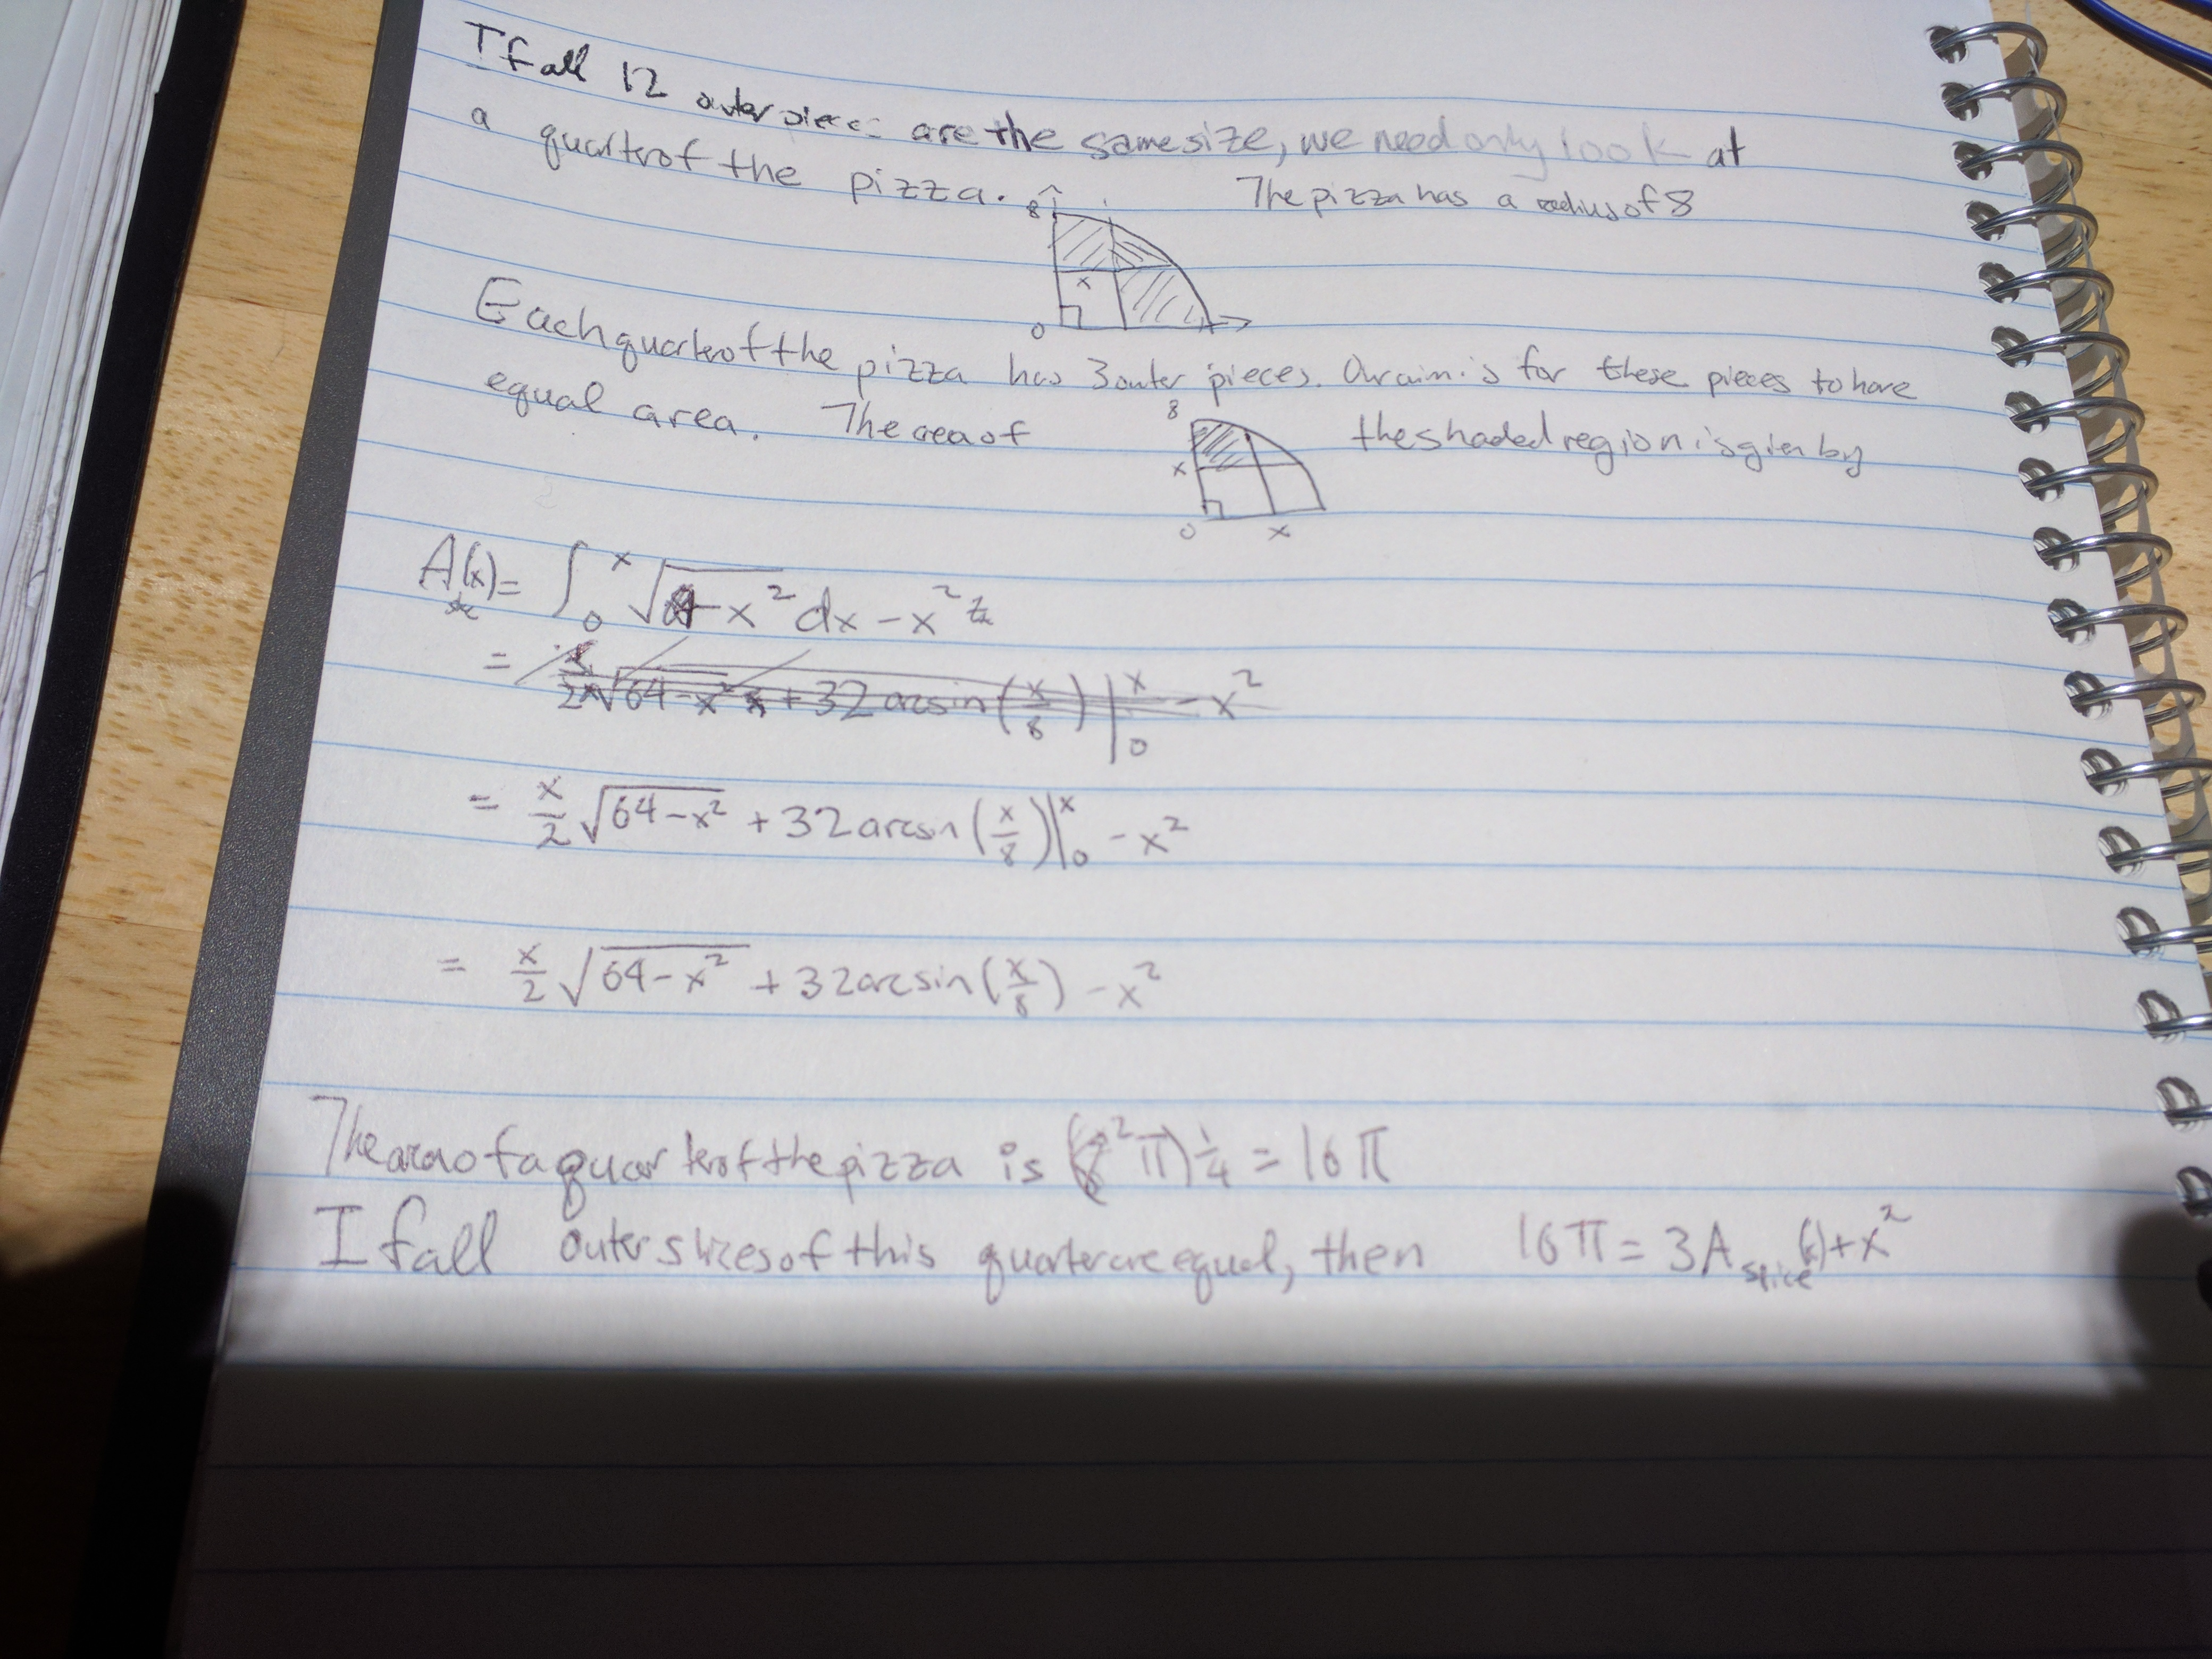
\includegraphics[width=.75\textwidth]{pizza}

\section{Doing Laundry}
Completely Done
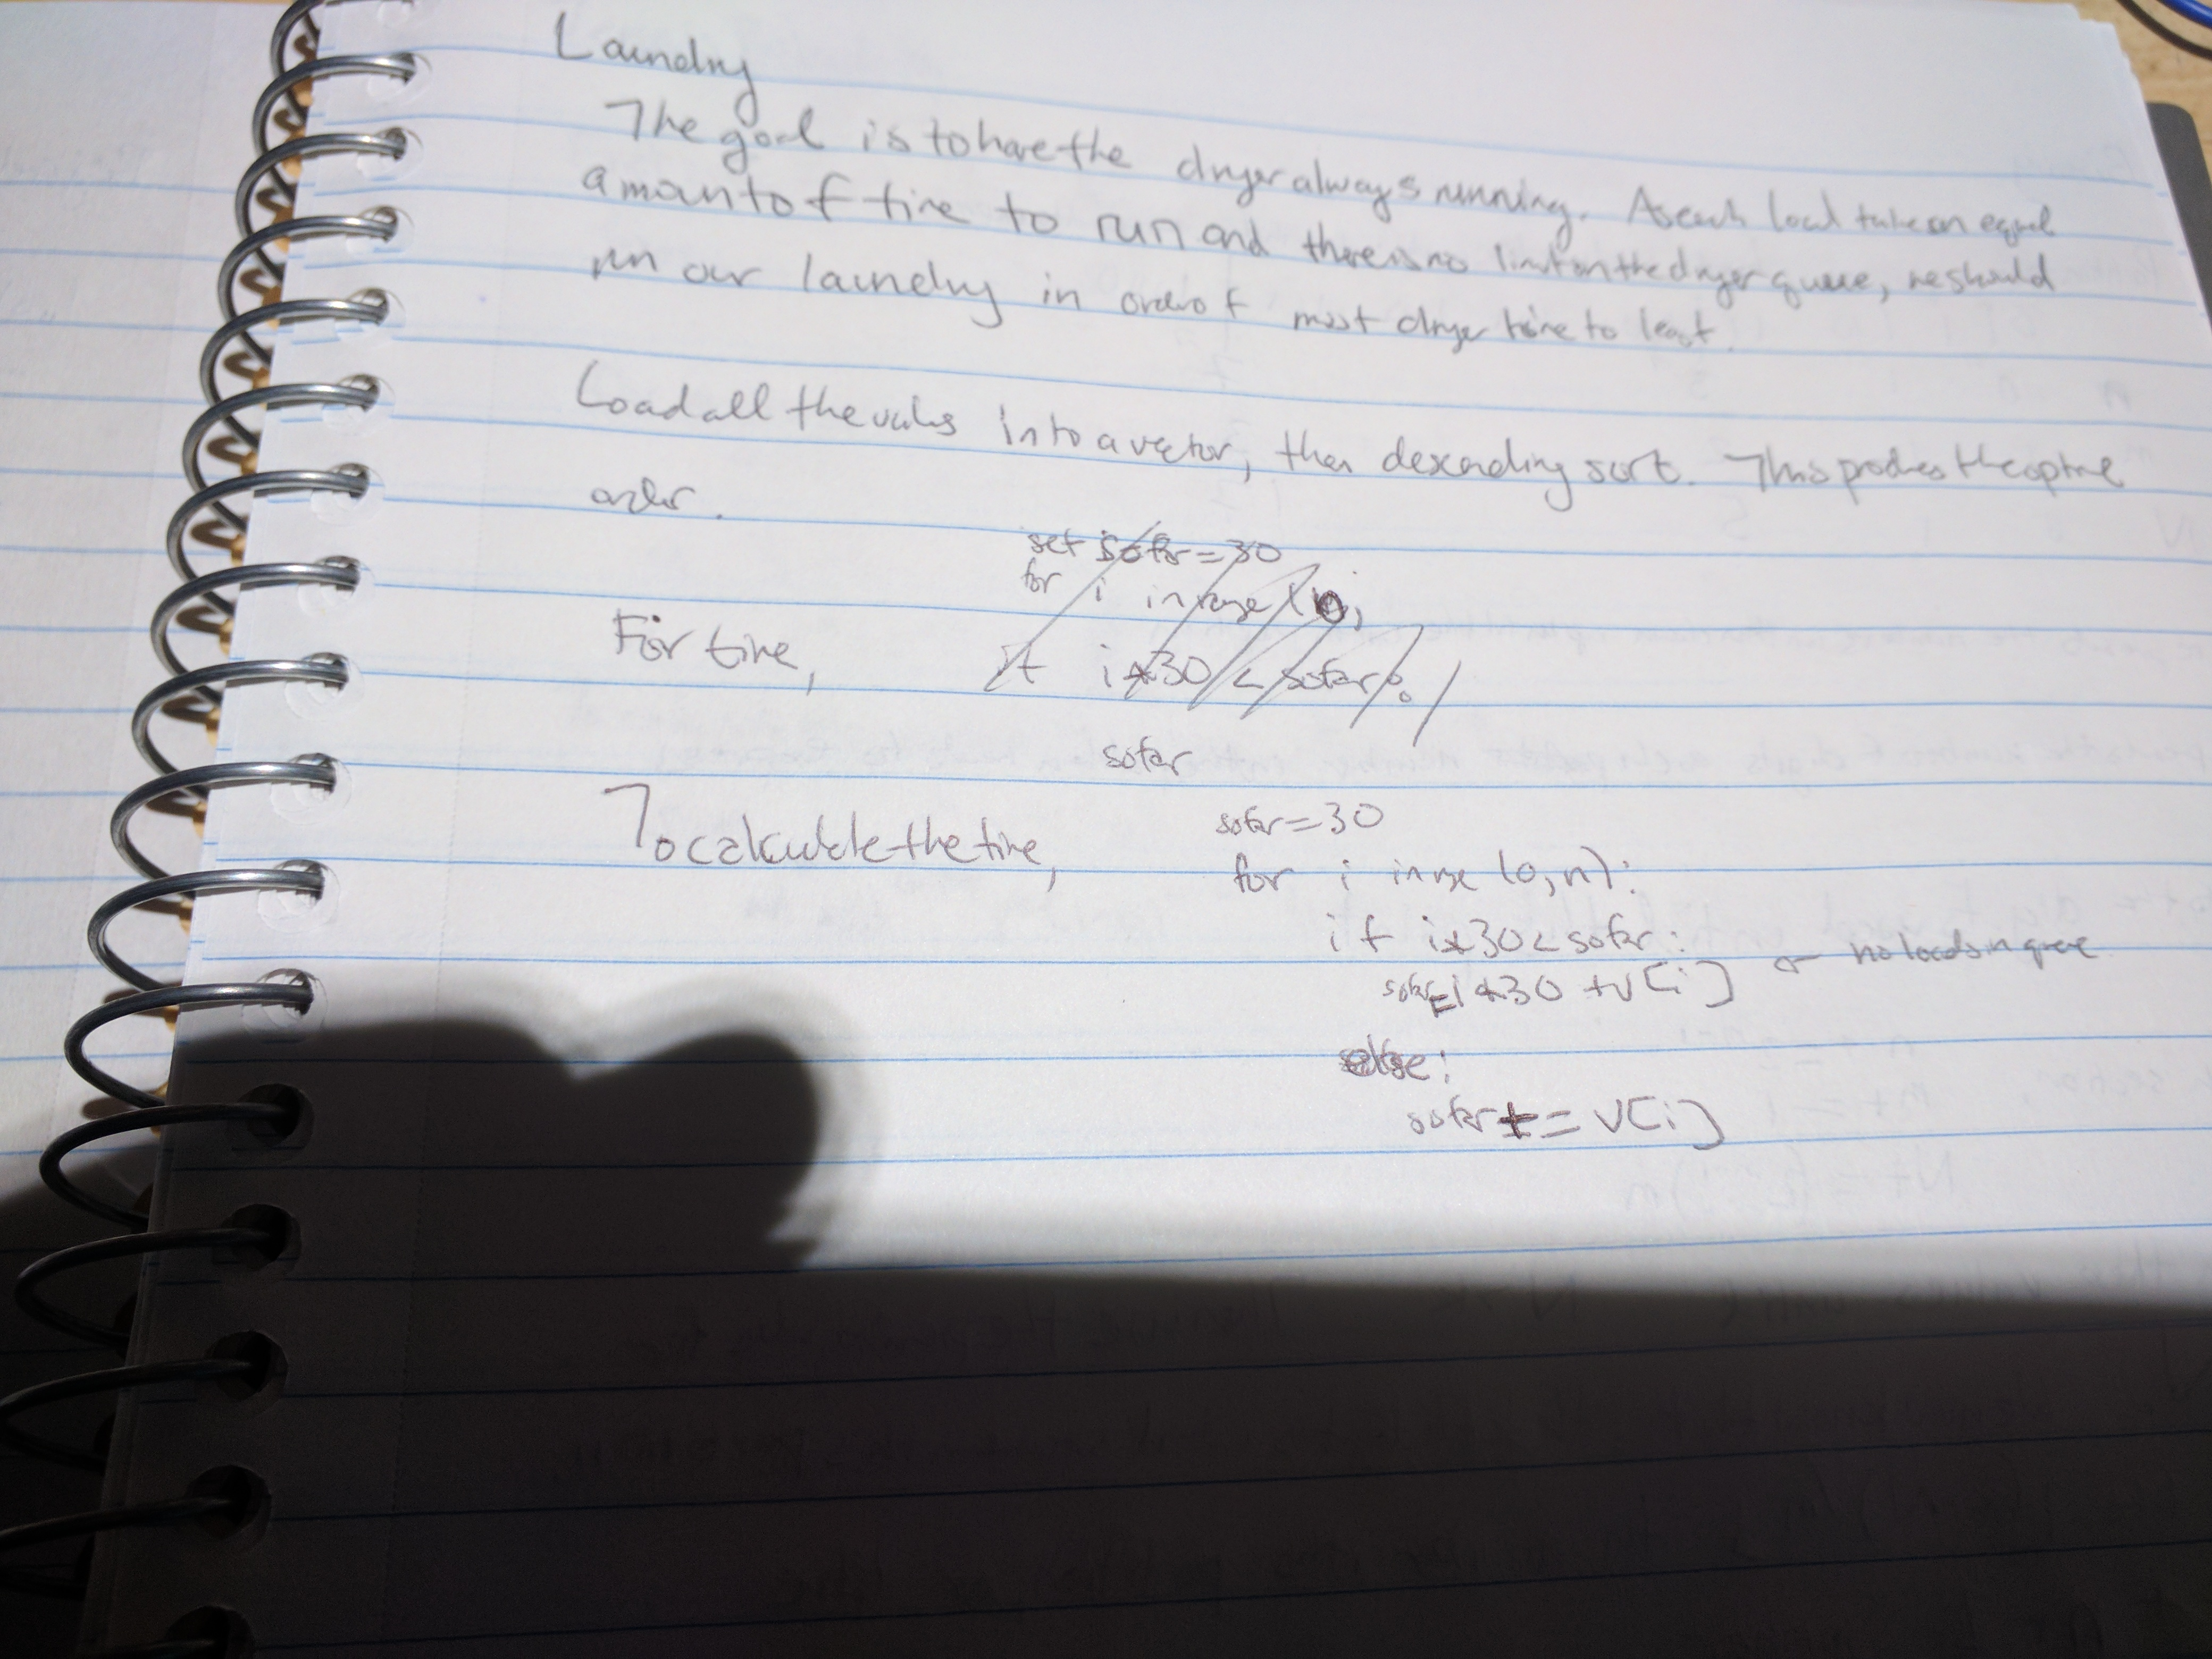
\includegraphics[width=.75\textwidth]{laundry}

\section{Linking Logos}
Kinda solution?

Partitions of n not hard to form. Create a bitmask of possible sums, with 1 where a break between two blocks would be. AND to see if there would be a disconnect. (needs pruning for time)

\section{Longshot}
Crappy solution, mostly done
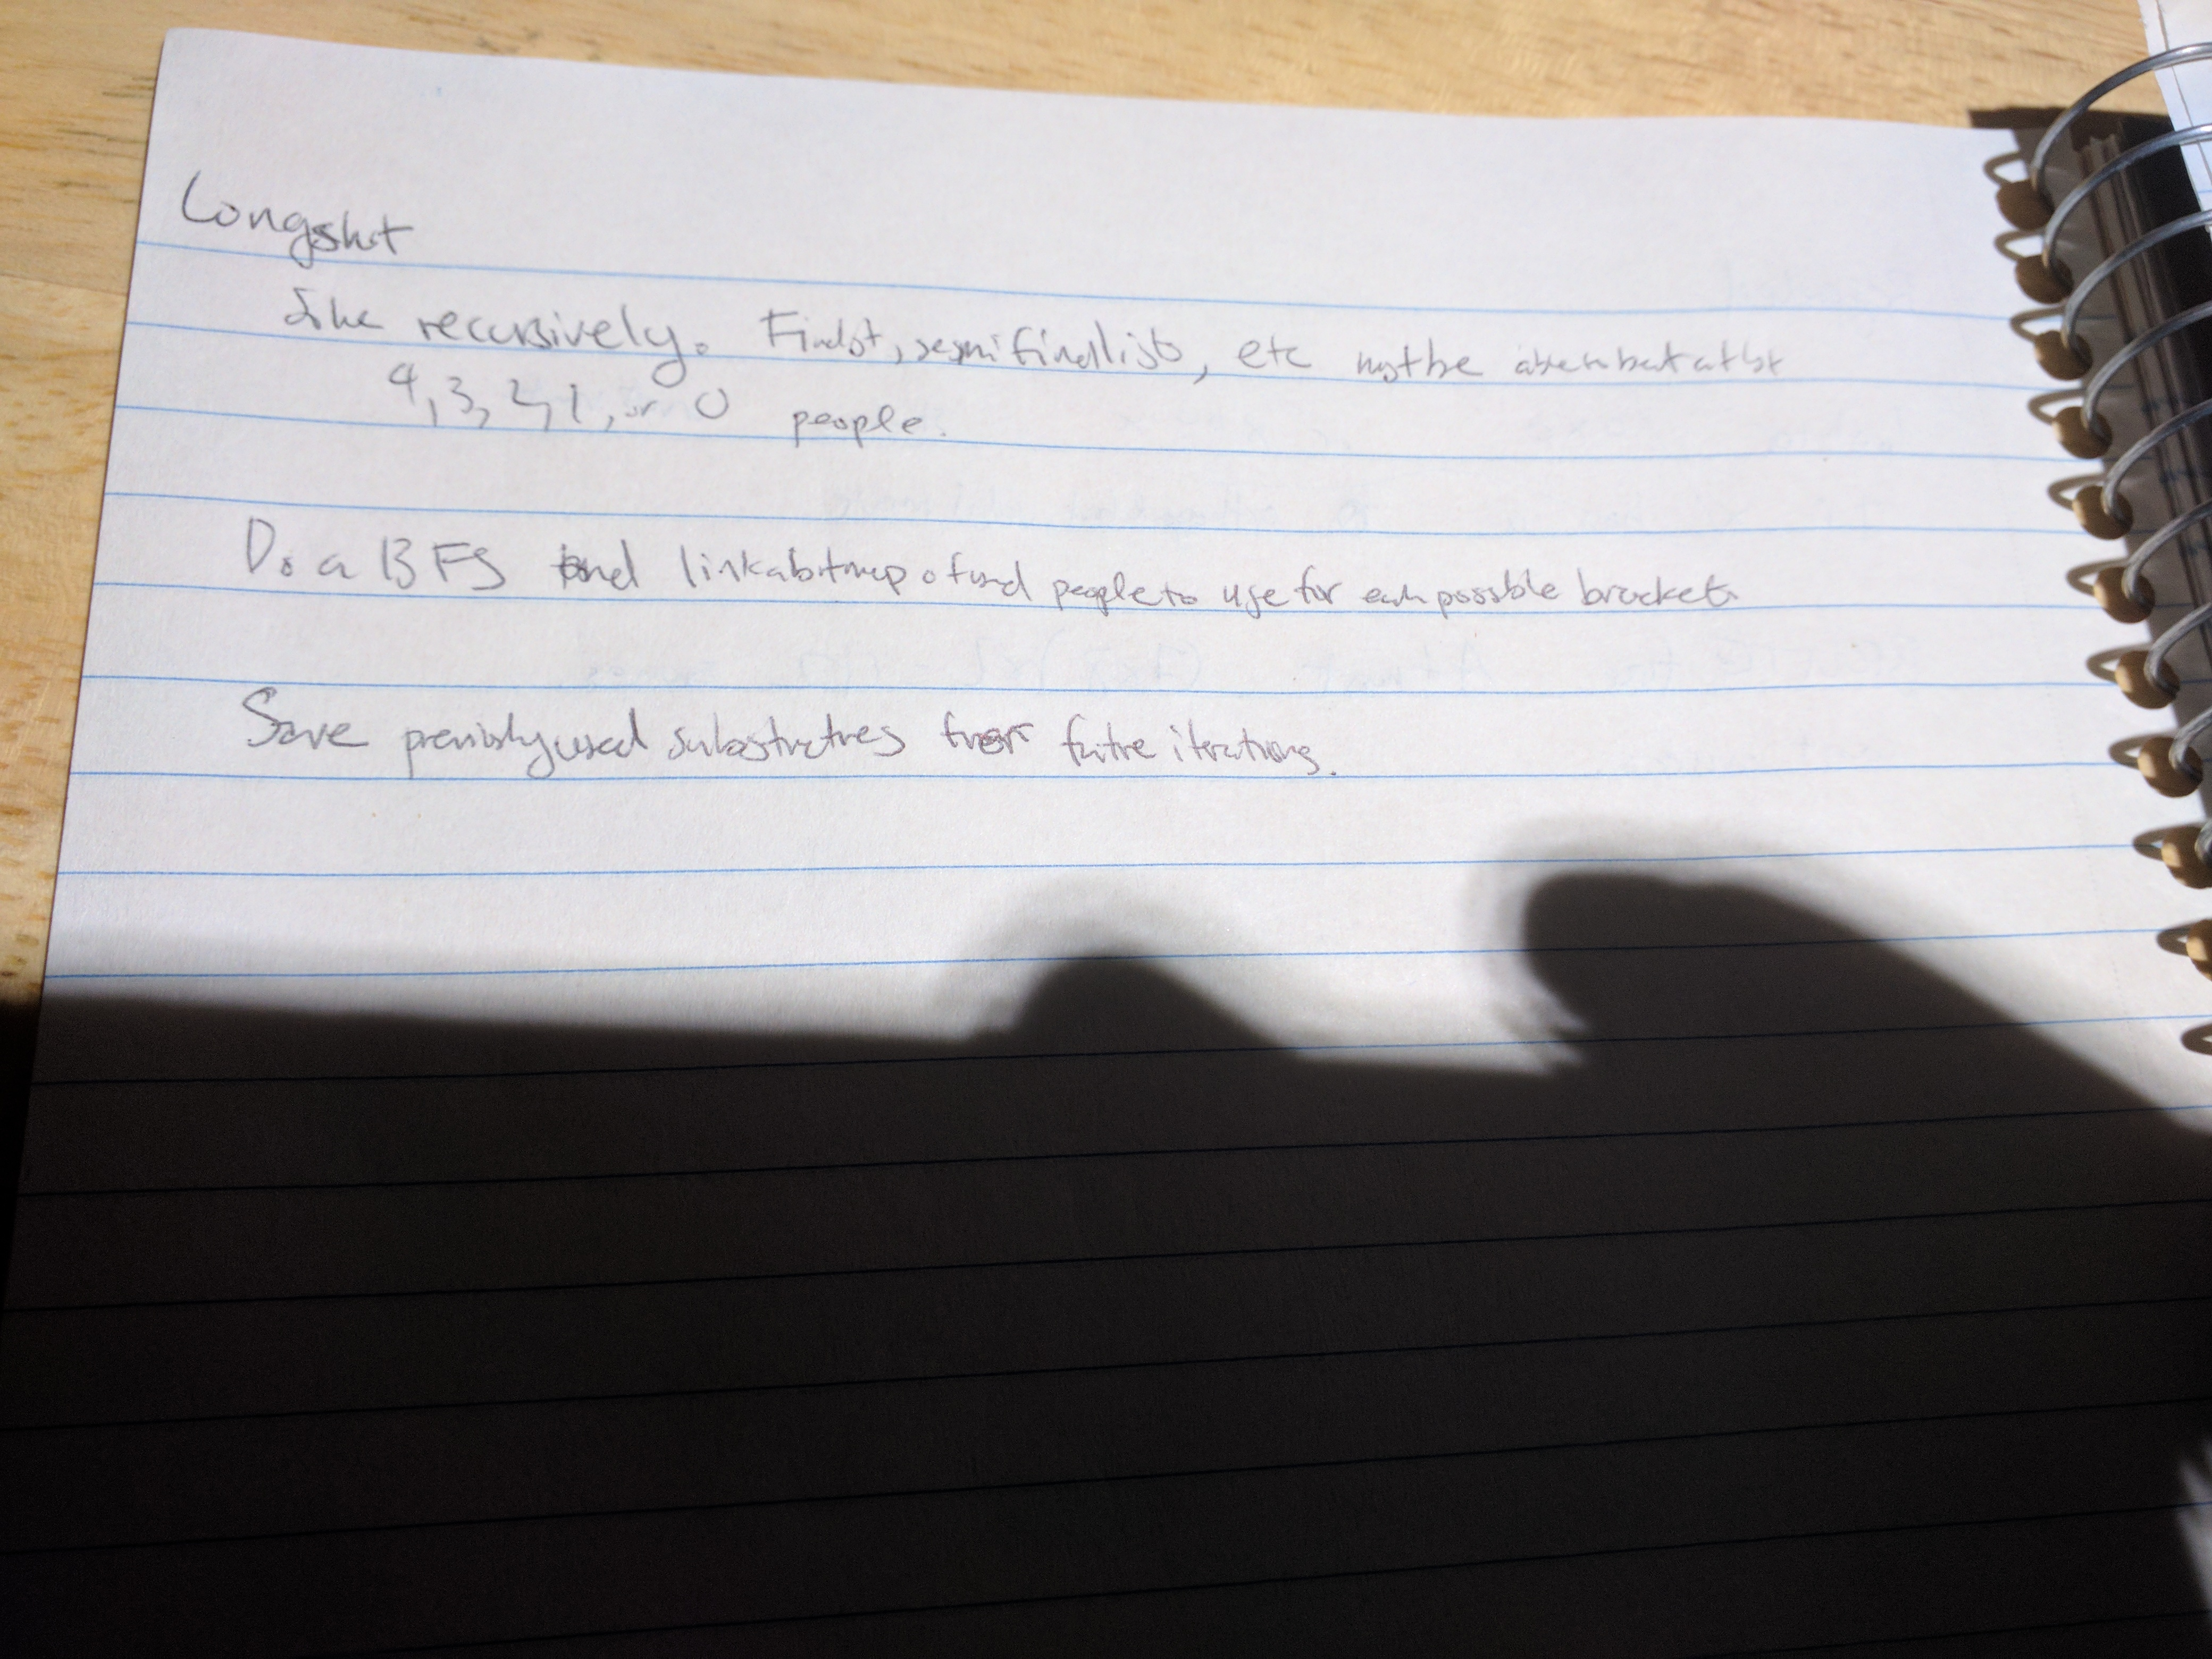
\includegraphics[width=.75\textwidth]{longshot}

\section{Prefix Goodness}
Suffix arrays. Ew. number of strings n is very large.

\section{Quantum Teleporters}
Shortest path problem from hell. Simple graph, but not a tree.


\section{Tennis Probability}
Completely Done
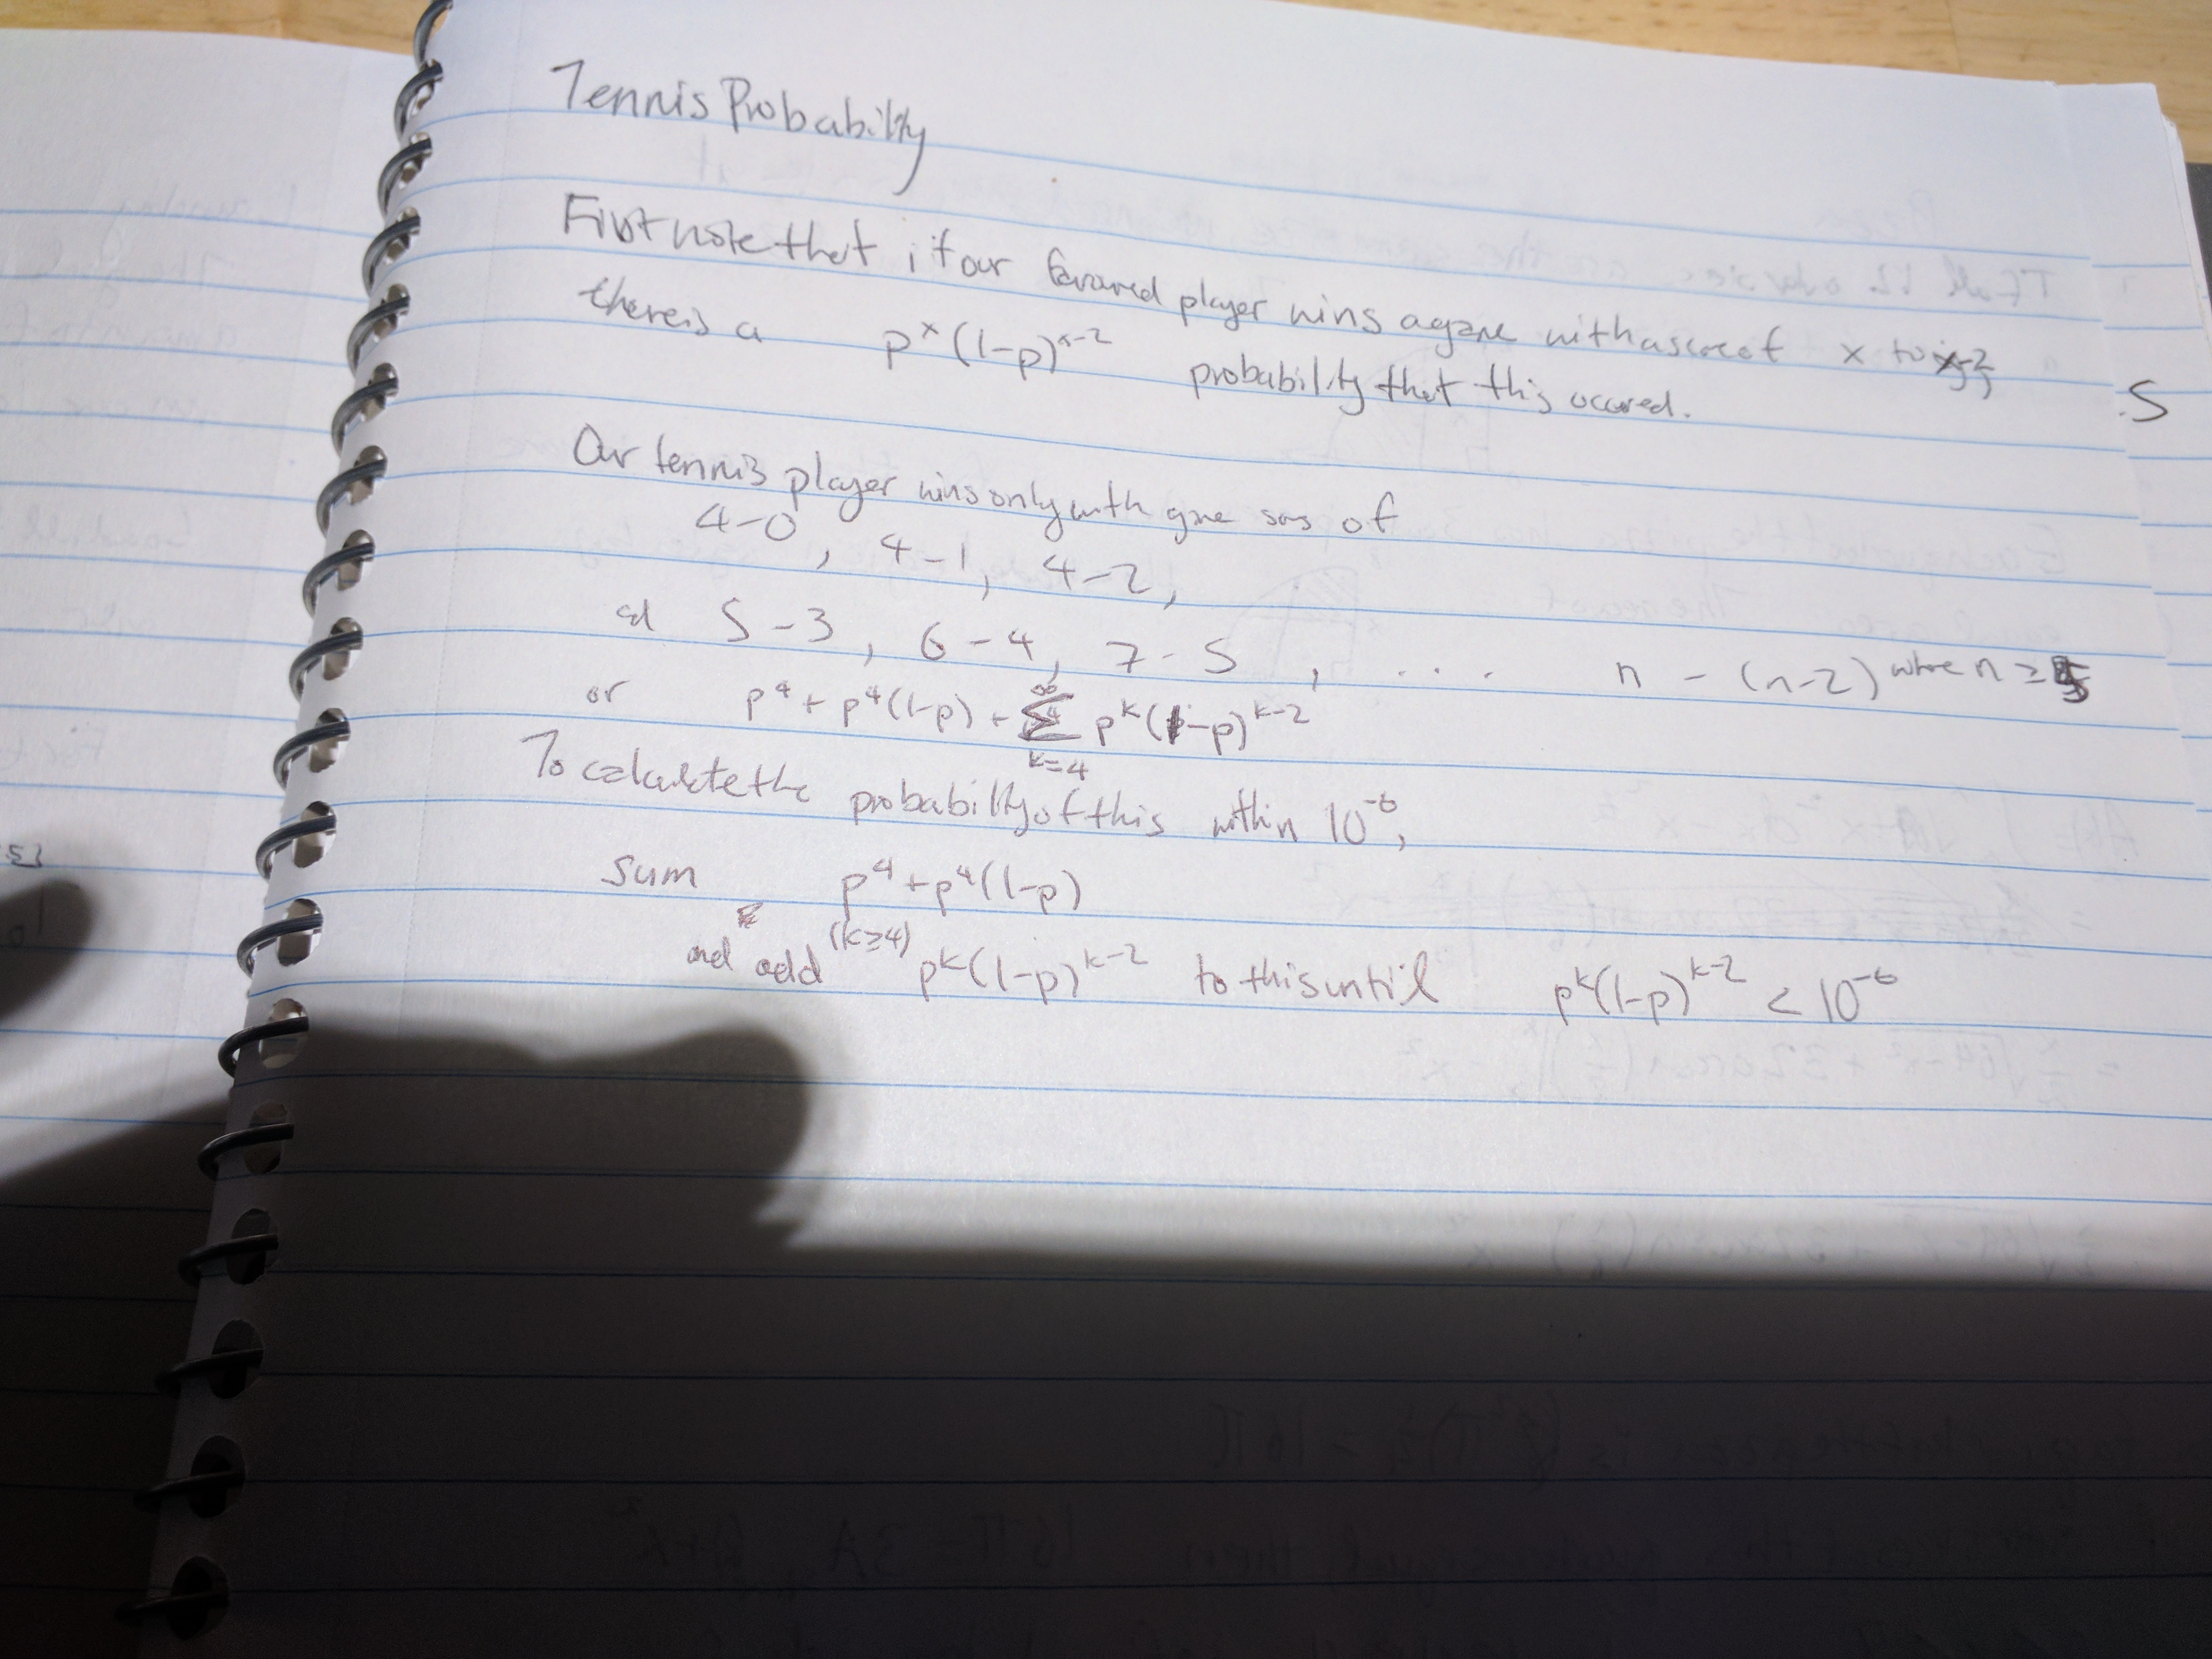
\includegraphics[width=.75\textwidth]{tennisprob}

\section{Zurch Trees}
Divide and conquer or something. Basically, the strategy is to leave an officer at stars and have an officer search the connected nodes. If this strategy is optimal, we just need some way of counting 'star depth'



\end{document}